\subsection{Setup ownCloud 7}

\initmarginpar{%

\includegraphics[width=0.8\marginparwidth]{owncloud2_logo}
\begin{flushright}
\scriptsize{ownCloud 2 Logo, Author ownCloud, AGPL}
\end{flushright}}

\begin{figure}[htp]
\centering
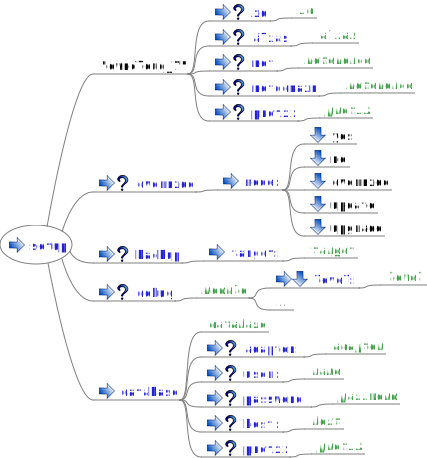
\includegraphics[width=0.7\textwidth]{httpd_setup_owncloud_7_script}
\label{fig:httpd_setup_owncloud_7_script}
\caption{Httpd ownCloud 7 Statements}
\end{figure}

%% setup owncloud_7
\TheStatement[httpd:domain:setup-owncloud_7]{setup "owncloud\_7"}
\TheStatement*[httpd!domain!setup!owncloud\_7]{setup "owncloud\_7" [, \Arg{id}] [, \Arg{alias}] [, \Arg{ref}] [, \Arg{refdomain}]}\\
\Statement{[, \Arg{prefix}], \{ override backup debug database \}}

Installs the ownCloud\footnote{\url{https://owncloud.org/}} browser-based
file sharing and synchronization service.

\begin{lstlisting}[style=Java]
httpd {
    domain "test1.com", address: "192.168.0.50", {
        setup "owncloud_7", alias: "/owncloud", {
        }
    }
}
\end{lstlisting}

%% override
\TheStatement[httpd:domain:setup-owncloud_7-override]{override}
\TheStatement*[httpd!domain!setup!owncloud_7!override]{override mode: \Type{yes} | \Type{no} | \Type{override} | \Type{update} | \Type{upgrade}}

Sets the override mode in case the service is already installed inside
the service prefix.
\begin{asparaitem}
\item \qcode{yes, override} to override the already installed service;
\item \qcode{no} never override the already installed service;
\item \qcode{update} override the already installed service only if the version is the same or newer;
\item \qcode{upgrade} override the already installed service only if the version is newer;
\end{asparaitem}

\begin{lstlisting}[style=Java]
httpd {
    domain "test1.com", address: "192.168.0.50", {
        setup "owncloud_7", alias: "/owncloud", {
            override mode: no
        }
    }
}
\end{lstlisting}

%% backup
\TheStatement[httpd:domain:setup-owncloud_7-backup]{backup}
\TheStatement*[httpd!domain!setup!owncloud_7!backup]{backup target: \Arg{target}}

Sets the \Arg{target} to where the service backups are stored.

\begin{lstlisting}[style=Java]
httpd {
    domain "test1.com", address: "192.168.0.50", {
        setup "owncloud_7", alias: "/owncloud", {
            backup target: "/var/backups"
        }
    }
}
\end{lstlisting}

%% debug
\TheStatement[httpd:domain:setup-owncloud_7-debug]{debug}
\TheStatement*[httpd!domain!setup!owncloud_7!debug]{debug \Arg{module}, level: \Arg{level} [, \dots]}

Sets the logging \Arg{level} and other parameters for the debug \Arg{module}.

\begin{lstlisting}[style=Java]
httpd {
    domain "test1.com", address: "192.168.0.50", {
        setup "owncloud_7", alias: "/owncloud", {
            debug "php", level: 1
            debug "owncloud", level: 1
        }
    }
}
\end{lstlisting}

%% database
\TheStatement[httpd:domain:setup-owncloud_7-database]{database}
\TheStatement*[httpd!domain!setup!owncloud_7!database]{database \Arg{database} [, user: \Arg{user}] [, password: \Arg{password}]} \\
\Statement{[, host: \Arg{host}] [, adapter: \Arg{adapter}]}

Sets the database use for the service.
\begin{asparaitem}
\item \Arg{database} the database name;
\item \Arg{user} optionally, the database user name;
\item \Arg{password} optionally, the user password;
\item \Arg{host} optionally, the database host;
\item \Arg{adapter} optionally, the database adapter;
\item \Arg{prefix} optionally, the table prefix;
\end{asparaitem}

\begin{lstlisting}[style=Java]
httpd {
    domain "test1.com", address: "192.168.0.50", {
        setup "owncloud_7", alias: "/owncloud", {
            database "ownclouddb", user: "userdb", password: "userpassdb", host: "localhost", adapter: "mysql"
        }
    }
}
\end{lstlisting}

\subsubsection{Httpd Owncloud 7 Examples}

Installs the ownCloud service in the speciefied domain.

\begin{lstlisting}[style=Sscontrol,
label={lst:owncloud_7_example_script_base},
title={Httpd.groovy}]
httpd {
    domain "test1.com", address: "192.168.0.51", {
        setup "owncloud_7", id: "owncloudid", alias: "/owncloud", prefix: "test1owncloud", {
            debug "php", level: 1
            debug "owncloud", level: 1
            override mode: OverrideMode.update
            backup target: "$tmp/var/backups"
            database "owncloud", user: "user", password: "userpass", host: "localhost", port: 3306, prefix: "owncloud_", adapter: "mysql"
        }
    }
    ssl_domain "test1.com", address: "192.168.0.51", {
        certificate file: certFile, key: certKeyFile
        setup "owncloud_7", ref: "owncloudid"
    }
}
\end{lstlisting}

Installs the ownCloud service in the speciefied domain with minimal configuration.

\begin{lstlisting}[style=Sscontrol,
label={lst:owncloud_7_example_script_minimal},
title={Httpd.groovy}]
httpd {
    domain "test1.com", address: "192.168.0.51", {
        setup "owncloud_7", {
            database "owncloud", user: "user", password: "userpass"
        }
    }
}
\end{lstlisting}

